% Chapter 2

\externaldocument{chapter3}
\externaldocument{chapter4}
\externaldocument{chapter5}
\externaldocument{chapter1}
\chapter{Formalisms} % Main chapter title

\label{Chapter2} % For referencing the chapter elsewhere, use \ref{Chapter2} 


%----------------------------------------------------------------------------------------

%\section{Welcome and Thank You}
%In this chapter, acoustical characteristics of music signal that enables general MIR tasks will be introduced.We will examine the Fourier Series representations of sound waves and see how they relate to harmonics and tonal color of instruments  



%----------------------------------------------------------------------------------------

\section{Representation of music signal}

The general aim of Music Information Retrieval (MIR) is to extract information about it's discriminants from the observed data. This observed signal is traditionally represented in the time domain. The time domain is a record of what happened to a parameter of the system versus time. Standard formats use amplitude versus time. The observed signal is then discretised by sampling and stored in digital format (see \ref{sampling}). This signal in the time domain is then changed to frequency domain. This is simply because our ear-brain combination is an excellent frequency domain analyser. Our brain splits the audio spectrum into many narrow bands and determines the power present in each band. Conversion from time domain to frequency domain is done using the foundations from \textit{Fourier theorem} (see \ref{time}). Currently used music signal representations for general MIR tasks are explained in section \ref{stft}.


\subsection{Sampling of continuous-time signal}
\label{sampling}
The digital formats contain the discrete version of the signal obtained by sampling continuous-time signal. Let $s(t)$ be a continuous function (or "signal") to be sampled, and let sampling be performed by measuring the value of the continuous function every T seconds, which is called the sampling interval or the sampling period. The sampling frequency or sampling rate, $f_{s}$, is the average number of samples obtained in one second (samples per second),  
\[
 f_{s} = \frac{1}{T}.
\]
The optimum sampling rate is given by Nyquist-Shannon sampling theorem which says, the sampling frequency $f_{s}$ should be at least twice the highest frequency contained in the signal. Given the human hearing range lies between 20Hz - 20KHz, most of the digital audio formats use a standard sampling frequency of 44.4Khz. The signal is further down sampled depending on the kind of feature information needed for classification. 


\subsection{Time-Frequency transformations}
\label{time}
The signal represented in the time domain is a set of ordered \textit{n}-tuples of real numbers \( (a_{1},a_{2}, ...,a_{N}) \in \mathbb{R}^N \) in the vector space \textit{V} , specifically \textit{Euclidean n-space}. That is to say, a discrete-time signal can be represented as a linear combination of Cartesian basis vectors. 
\begin{equation}
\textbf{a}(t) = (a_{1},a_{2}, ...,a_{N}) = a_{1}\textbf{e}_{1} + a_{2}\textbf{e}_{2} + ... + a_{N}\textbf{e}_{N} = \displaystyle\sum_{i=1}^{N}a_{i}\textbf{e}_{i}
\end{equation} 
where:\\
\indent \textbf{a} is a discrete-time signal\\
\indent $\textbf{e}_{1} ... \textbf{e}_{N}$ are Cartesian basis vectors (Unit vectors).
\bigskip

\noindent Mapping from time-domain to frequency-domain is looked up on as basis transformation. We need to find a set of basis vectors $\bm{\phi}_{ \omega }$, whose coefficients $c_{ \omega }$ then represents the components in frequency domain. 
\begin{equation}
\label{exp_fourier}
\textbf{a}(t) = \displaystyle\sum_{ \omega =0}^{M-1}c_{ \omega }\bm{\phi}_{ \omega }(t) 
\end{equation}
for some integer $0 < M < \infty$. Then $\textbf{c}(\phi) = (c_{0},c_{1}, ...,c_{M-1}) \in \mathbb{C}^M $ represents the components in frequency domain. Thus our aim is to compute $\textbf{c}(\phi)$ by defining basis vectors $\bm{\phi}_{\omega}$ which are functions of frequency. Computing the Fourier coefficients for periodic and aperiodic signals are discussed below.

\subsubsection{Periodic Signals}
If $\textbf{a}(t)$ is periodic in \textbf{T}, then we can apply the definition of \textbf{Exponential Fourier Series} expansion and define $\bm{\phi}$ in equation \ref{exp_fourier} as,
\begin{equation}
\bm{\phi}_{k}(t) = \frac{1}{\sqrt{T}}e^{ik \omega t}
\end{equation}    
Whose basis functions $\bm{\phi}$ now form \textit{complete orthonormal} set \cite{allen}. That is, 
\begin{equation}
\label{ortho}
 < \bm{\phi}_{i}, \bm{\phi}_{j} > =
	\begin{cases}
	  0 & i \neq j \\
	  1 &  i = j \\ 
	\end{cases}
\end{equation}
The fourier series finds a set of discrete coefficients of \textbf{harmonically related frequencies} $(k \omega )$ . To retrieve $c_{k}$, multiply $\bm{\phi}_{k}$ on both sides of equation \ref{exp_fourier} and apply the conditions of orthonormality in equation \ref{ortho}. Thus
\begin{equation}
c_{k} = <\textbf{a}(t), \bm{\phi}_{k}(t)>
\end{equation}


\subsubsection{Aperiodic Signals}
It is difficult to assume periodicity for a generalized signal. We need to estimate the coefficients $\textbf{c}$ for continuous frequency variable $\bm{\omega}$ instead of discrete harmonics $\textbf{k}\bm{\omega}$. The Fourier series can not be applied directly and hence Fourier Transform was developed. Here we aim to find out quantity of each sinusoids is the signal $\textbf{a}(t)$. This can be done by dividing  $\textbf{a}(t)$ by $e^{i \omega t}$ over the time domain. Thus, the coefficients in the frequency domain are 
\begin{equation}
c_{\omega} =  \displaystyle\sum_{t=0}^{N-1}a(t)e^{-i \omega t}
\end{equation}  
This is the N-point \textbf{Discrete Fourier Transform}. For the proof of existence of such coefficients, please refer to chapter ?? in \cite{allen}. \textbf{Fast Fourier Transform}(FFT) is an efficient implementation of Discrete Fourier Transform(DFT) which exploits the symmetry of $sines$ and $cosines$. While DFT requires $O(N^2)$ operations, FFT requires only $O(NlogN)$ \cite{allen}.  

\subsection{STFT, Mel-Spectrogram}
\label{stft}
It is useful to perform FFT locally over short segments. This is because we are more interested in the evolution of frequency content rather than the frequency content of the entire signal. Hence, the full length signal is divided into short segments, and FFT is computed separately for each segment. This is known as \textbf{Short Time Fourier Transform (STFT)}. To avoid \textit{spectral leakage}, the original signal is modified by applying some window function. The most common window function is the \textbf{Hamming Window} defined as,
\begin{equation}
h[n] = 0.54 - 0.46cos(\frac{2 \pi n}{N-1})
\end{equation}
Where $n \in {0,1,...,N-1}$. The signal approaches zero near $n=0$ and $n=N-1$, but reaches peak near $n=N/2$ \cite{specLeak}. To overcome the information loss at the ends of the window, signal is divided into segments that are partly \textit{overlapping} with eachother. Figure \ref{fig:stftPipe} shows the extraction of spectral frames of a spectrogram.  
\begin{figure}[h]
       \begin{subfigure}[b]{0.6\textwidth}
        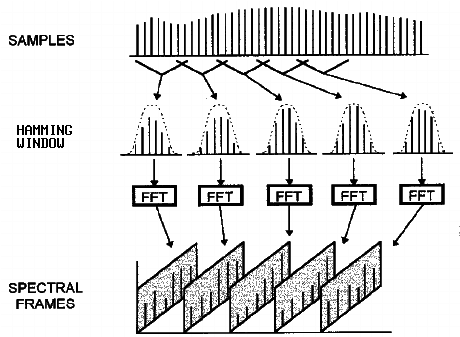
\includegraphics[width=\textwidth]{stft_pipe}
        \caption{Windowing is applied on overlapping segments\\ followed by FFT }
        \label{fig:stftPipe}
       \end{subfigure}
	    \begin{subfigure}[b]{0.4\textwidth}
        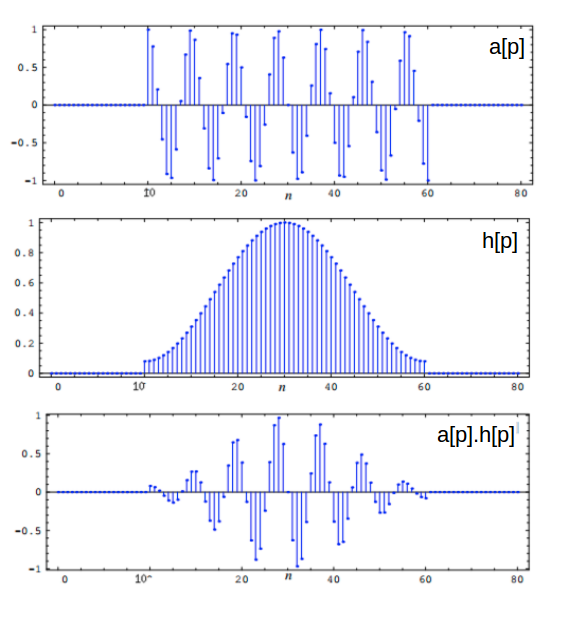
\includegraphics[width=\textwidth]{stft}
        \caption{
        Application of Hamming Window on \\a segment of input signal
        }
        \label{fig:HammingWindow}
       \end{subfigure}
       \caption{(a) Shows STFT Pipeline. (b) Shows the application of \\Window function}\label{fig:STFT}
\end{figure}
\bigskip

\noindent The discrete STFT (\textit{slow}) for $p^{th}$ frame of signal $\textbf{a}$ is obtained as,
\begin{equation}
\label{stfteq}
\textbf{C}(p, \omega ) = \displaystyle\sum_{n=p.s}^{p.s + F}\textbf{a}(n)\textbf{h}(n-p.s)e^{-i \omega (n-p.s)}
\end{equation}
Where:
\begin{itemize}[label=]
    \setlength\itemsep{0em}
    \item $P$: is the number of spectral frames; $p \in [0,1..P-1]$ 
    \item $M$: is the dimension of discrete frequency space ; $\omega \in \mathbb{R}^{M}$
    \item $F$: is the frame length 
    \item $s$: is stride (or) hop-length for the next segment
    \item $\textbf{a} \in  \mathbb{R}^{N}$ ; $n \in [0,1...N-1]$
    \item $\textbf{h} \in  \mathbb{R}^{F}$
    \item $\omega \in  \mathbb{R}^{M}$
    \item $\textbf{C}$: is Fourier Coefficient Matrix ; $\textbf{C} : \mathbb{R}^{F.P} \rightarrow \mathbb{C}^{M \times P}$
\end{itemize}

\noindent Equation \ref{stfteq} can be seen as a \textbf{convolution} over the signal \textbf{a} with \textbf{W} which has finite support over the set $\left\{0,1..,F \right\}$
\begin{equation}
\boxed
{
  \textbf{C}(p, \omega ) = \textbf{a}(n) \star \textbf{W}_{\omega}(n- \tau)
}
\end{equation}
Where:
\begin{itemize}[label=]
    \setlength\itemsep{0em}
    \item $ \tau$ = $p.s$
    \item $\textbf{W}_{\omega}(n- \tau)$ = $\textbf{h}(n- \tau )e^{-i \omega (n- \tau)}$
\end{itemize}
It is important to note that the coefficients $c_{\omega}$ may be complex valued. To obtain useful metrics, we need to extract some physical quantity from the coefficients. This is where \textbf{Parseval's theorem} is used, which relates and time and frequency domain components in DFT as follows \cite{allen} :
\begin{equation}
{\|\textbf{c}\|}^2 \propto {\|\textbf{a}\|}^2
\end{equation}
If \textbf{a} represents amplitude in the time-domain, then as a consequence of Hook's law  on energy equation, we know that
\begin{equation}
Energy \propto amplitude^2
\end{equation}
Relating equation 2.11 and 2.12, it can be inferred that \textbf{square} of the Fourier coefficients is proportional to the energy distributed in the corresponding frequencies. This is called the \textbf{Power Spectrum (E)}. It is often motivating to use this representation because \textit{loudness} is proportional to \textit{energy}.
\begin{equation}
\label{energy}
\textbf{E} = \textbf{C} \odot \textbf{C}
\end{equation}

\noindent The frequencies in the considered range are  grouped into bins. It is useful to do so, not only to reduce dimension but also due to the aliasing effect of human auditory system. This is motivated by the human cochlea (an organ in the ear) which vibrates at different spots depending on the frequency of the incoming sounds.
  
\subsubsection{Mel Spectrogram}
\label{mel}

The \textit{mel-scale} was developed to express measured frequency in terms of psychological metrics (i.e perceived pitch). The mel-scale was developed
by experimenting with the human ears interpretation of a pitch. The experiment showed that the pitch is linearly perceived in the frequency range 0-1000 Hz. Above
1000 Hz, the scale becomes logarithmic. There are several formulae to convert Hertz to mel. A popularly used formula is noted in \cite{speech}
\begin{equation}
\omega_{m} = 2595log_{10}\bigg(1+\frac{ \omega }{700}\bigg)
\end{equation}
Where $\omega$ is the frequency in Hertz. In a mel spectrogram, the frequencies and converted to mels and then grouped into mel-spaced bins. This is done by multiplying the spectrum with some \textbf{filter bank ($\textbf{M}_{\omega_{m}}$)}. For details about computation of mel-filter banks, refer \cite{mel}. Each filter bank is centered at a specific frequency. Hence, to compute R mel bins, we need R mel-filter banks. 
\begin{equation}
\label{mel_conv}
\textbf{Mel}(p,\omega_{m}) = \displaystyle\sum_{ \omega = 0}^{M}\textbf{Y}(p, \omega)\textbf{M}_{\omega_{m}}(\omega)
\end{equation}
Where:
\begin{itemize}[label=]
    \setlength\itemsep{0em}
    \item $\textbf{Y}$ = $f(\textbf{C})$
    \item $\omega_{m}$ = mel frequency
\end{itemize}    
When the function $f$ is an defined by equation \ref{energy}, we get \textbf{mel power spectrogram}
\bigskip

\noindent We can re-write equation \ref{mel_conv} as, 
\begin{equation}
\label{mel_conv_flat}
\textbf{Mel}(p,\omega_{m}) = \displaystyle\sum_{k=p.M}^{p.M + K}\textbf{U}(k)\textbf{M}_{\omega_{m}}(k-p.M)
\end{equation}
Where:
\begin{itemize}[label=]
    \setlength\itemsep{0em}
    \item $\textbf{Mel}$: is Mel Spectrum Matrix ; $\textbf{Mel} : \mathbb{R}^{M.P} \rightarrow \mathbb{R}^{R \times P}$
    \item $P$: is the number of spectral frames; $p \in [0,1..P-1]$ 
    \item $M$: is the dimension of discrete frequency space ; $\omega = k-p.M \in \mathbb{R}^{M}$
    \item $K$ = $M.P$ and $k \in [0,1...K]$
    \item $\textbf{U}(k)$ = $\textbf{Y}(i,j)$ ; $i = floor(\frac{k}{M})$ ; $j = k-floor(\frac{Mk}{M-1})$
    \item $\textbf{Y} \in \mathbb{R}^{M \times P}$
    \item $\textbf{U} \in \mathbb{R}^{M.P}$
    \item $\omega_{m} \in  \mathbb{R}^{R}$
\end{itemize}

\noindent Hence, we can represent mel-spectrogram as \textbf{M-strided convolution} over \textit{flattened} $\textbf{Y}$ with mel filters $\textbf{M}_{\omega_{m}}$ (i.e, the frequency axis of $\textbf{C}$ is contracted with each mel-filter, 
\begin{equation}
\boxed
{
  \textbf{Mel}(p, \omega_{m} ) = \textbf{U}(k) \star \textbf{M}_{\omega_{m}}(k - p.M)
}
\end{equation}
  
\bigskip

\section{Dimensionality Reduction}
\label{dimension}
The objective of dimensionality reduction is to retain only the information that contribute to discrimination and discard the rest. This is done because the representation ($\textbf{R}$) can be large for longer audio tracks (because number of frames $P$ depends on length of the audio). Reduction over a large frame at once can lead to loss of temporal information. Hence, dimensionality reduction is done hierarchically, sometimes by stacking combination of these techniques. We generalize the operations on input signal $\textbf{a}$ as follows,
\[
   \textbf{R} = Rep(\textbf{a}) \qquad Rep : \mathbb{R}^{N} \rightarrow \mathbb{R}^{R \times P}
\]
\[
   \textbf{X} = f(\textbf{R}) \qquad f : \mathbb{R}^{R \times P} \rightarrow \mathbb{R}^{S \times Q} 
\]
\begin{equation}
\label{dim_red_abstract}
   \textbf{Y} = D(\textbf{X}) \qquad D : \mathbb{R}^{S \times Q} \rightarrow \mathbb{R}^{T \times W} 
\end{equation}
 

\noindent The representation operations defined in the previous section can be a part of the function $Rep$. Since dimension reductions can be stacked, $f$ represents the previous reductions applied. $Q$ and $W$ are number of frames as a result of hierarchical windowing operation shown in fig \ref{fig:Dimensionality Reduction}. For the first reduction however, $f$ does not exist and hence represented by conditional arrow (dotted). The output of reduction $\textbf{Y} \in \mathbb{R}^{T \times W}$ will then be the reduced representation ($T < S$ or $W < Q$). Depending on how the function $D$ is defined, we will classify the techniques into broad categories.
\begin{itemize}
  \item Reduction by basis transformation
  \item Reduction by stacked convolutions
  \item Reduction by clustering 
\end{itemize} 
\begin{figure}[h] 
\centering
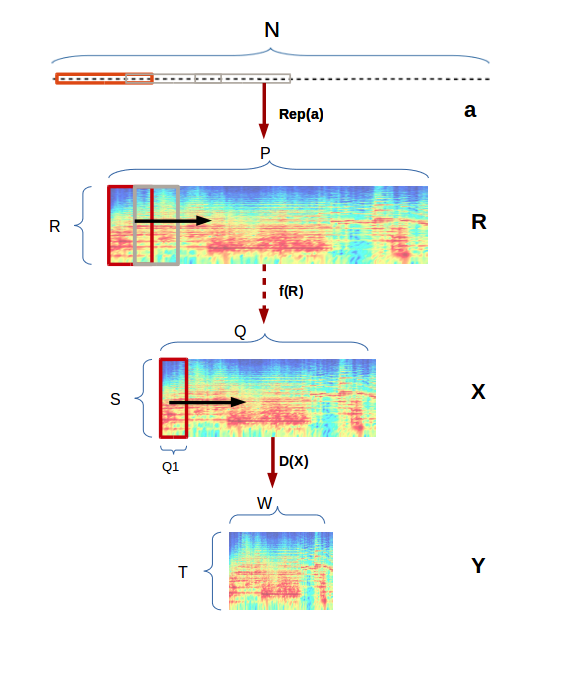
\includegraphics[width=0.5\textwidth]{dim_red}
\caption{Dimensionality Reduction Pipeline}
 \label{fig:Dimensionality Reduction}
 \end{figure}
\FloatBarrier
\bigskip

\subsection{Basis Transformations - PCA, MFCC}
\label{basis}

The basis vectors are functions of the properties we want to encode. In equation \ref{exp_fourier}, we used basis transformation to represent the signal in frequency domain. Now we want to use the same concept, but for dimensionality reduction. In general terms, this is done by changing to a reduced basis. That is, we need to find a change of coordinates matrix that will map the input to a basis system with lesser coordinates. 
\bigskip

\noindent The input frame $\textbf{X}_{w}$ is first operated with some window function $\textbf{w}$ involving statistical operation,
\[
  \textbf{z}_{w} = \{\textbf{X}_{w}\textbf{w} \quad | \quad \textbf{X}_{w} \in \mathbb{R}^{S \times J}, \textbf{w} \in \mathbb{R}^{J}, \textbf{z}_{w} \in \mathbb{R}^{S}\}
\]    
Now we have to compute $\textbf{y}_{w} \in \mathbb{R}^{T}$ which has least representation error with $\textbf{z}_{w} \in \mathbb{R}^{S}$ such that $T < S$. Let us say, $\textbf{z}_{w}$ can be written as a linear combination of some basis $\textbf{V} = [\textbf{v}_{1}, \textbf{v}_{2}, ..,\textbf{v}_{T}] \in \mathbb{R}^{S \times T}$ with coordinates $\textbf{y}_{w} = [y_{1}, y_{2},...,y_{T}]$. Then $\textbf{y}_{w}$ can be calculated by solving,
\[
\textbf{z}_{w} = \displaystyle\sum_{i=1}^{T}y_{i}\textbf{v}_{i} = \textbf{V}\textbf{y}_{w}
\]
\[
\textbf{y}_{w} = \textbf{V}^{-1}\textbf{z}_{w}
\]
Thus, the operator $D$ in equation \ref{dim_red_abstract} is,
\[
\textbf{Y} = D(\textbf{X}, \textbf{V})
\]
Therefore, dimension reduction through basis transformation are those class of techniques where $D$ is a function of some invertible change of coordinates matrix $\textbf{V}$. Now, depending on how $\textbf{V}$ is defined, some methods are discussed.

\subsubsection{Principal Component Analysis (PCA)}
The frequencies in the adjacent bins can be highly correlated and therefore contain redundant information. Principal component Analysis is a procedure to transform large number of correlated variables into smaller number of uncorrelated variables. Moreover, only the information corresponding to high variance basis contributes to discrimination. This means, $\textbf{y}_{w}$ should be approximated with basis vectors that account for large variance. Hence, in PCA based techniques, dimension reduction is done through basis vectors of covariance matrix ($\bm{\Sigma}$). The coordinates of the resulting basis system are known as \textit{principal components}. The steps of this abstraction are enumerated,
\begin{enumerate}[label=(\alph*)]
\item Usually, large samples of inputs are concatenated to compute the covariance matrix. The rows of $\textbf{X}$ are centred by their mean and covariance is computed as,
\[
   \bm{\Sigma} = \textbf{E}[(\textbf{X} - \textbf{E}[\textbf{X}])(\textbf{X} - \textbf{E}[\textbf{X}])^{T}] = \frac{1}{Q}\textbf{\^X}\textbf{\^X}^{T} \quad \in \mathbb{S}^{S \times S}
\]
\item The eigen values and eigen vectors of $\bm{\Sigma}$ are computed. At this point, we use the Orthogonal Eigenvector Decomposition Theorem (see Appendix ??) and infer that eigen vectors of symmetric matrix ($\bm{\Sigma}$) form an orthogonal basis in $\mathbb{R}^{S}$. 
\[
\bm{\Sigma} = \textbf{V}\bm{\Lambda}\textbf{V}^{T} \qquad \textbf{V} \in \mathbb{O}^{S \times S}, \quad \bm{\Lambda} \in \mathbb{D}^{S \times S}
\]

\item The eigen values represent the magnitude of variance for each frequency.  Hence, eigenvectors corresponding to large eigen values gives the coordinates corresponding to greater variance. So eigen vectors corresponding to top $T$ eigen values are retained, while ignoring coordinates of lower variance. The resulting change of coordinates matrix is then $\textbf{\^V} \in \mathbb{O}^{S \times T}$
   
\item Since $\textbf{\^V}$ is orthogonal, $\textbf{\^{V}}^{-1} = \textbf{\^{V}}^{T}$, and we can compute $\textbf{y}_{w} = \textbf{\^{V}}^{T}\textbf{z}_{w}$

\end{enumerate}   

\begin{algorithm}
  \caption{$\textbf{Y}$ = PCA($\textbf{X}$)}\label{PCA}
  \begin{algorithmic}[1]
    \Statex \textbf{Input :} $\textbf{X} \in \mathbb{R}^{S \times Q}$
    \Statex \textbf{Output :} $\textbf{Y} \in \mathbb{R}^{T \times Q}$
      \State $\bm{\Sigma} = \frac{1}{Q}\textbf{X}\textbf{X}^{T}$ \Comment{$\bm{\Sigma} \in \mathbb{S}^{S \times S}$}
      \State $\textbf{V}^{T} \bm{\Lambda} \textbf{V} = \bm{\Sigma}$ \Comment{$\bm{\Lambda} \in \mathbb{D}^{T \times T}$ , $\textbf{V} \in \mathbb{O}^{S \times S}$}
      \State $\textbf{V} \leftarrow \textbf{V}[:][:T]$ \Comment{$\textbf{V} \in \mathbb{O}^{S \times T}$}
      \State $\textbf{\^{X}} = \textbf{X} - \textbf{E}[\textbf{X}]$
      \State $\textbf{Y} \leftarrow \textbf{V}^{T}\textbf{\^{X}}$
  \end{algorithmic}
\end{algorithm}
\FloatBarrier
\bigskip

\noindent Sometimes, to make the resulting reduction $\textbf{Y}$ uncorrelated, the corresponding dimensions are divided by their eigen values. This is because eigen values are proportional to the magnitude of variance in each frequency direction. This operation is known as \textbf{PCA Whitening}   
\[
\textbf{Y} \leftarrow \bm{\Lambda}^{-1}\textbf{V}^{T}\textbf{\^{X}}
\]
\bigskip

\subsubsection{Mel-frequency cepstrum coefficients (MFCC)}
It has been studied that the spectral basis functions of cosine transform in mel-log power spectrogram are similar to the corresponding principal component basis[]. MFCC coefficients are obtained by taking discrete cosine transform of the mel log power spectrogram. Since these basis functions are similar to that of co-variance matrix, using the coefficients corresponding to high frequency cosine functions encodes the information corresponding to large variance. 
\begin{algorithm}
  \caption{$\textbf{Y}$ = MFCC($\textbf{a}$) }\label{MFCC}
  \begin{algorithmic}[1]
    \Statex \textbf{Input :} $\textbf{a} \in \mathbb{R}^{N}$
    \Statex \textbf{Output :} $\textbf{Y} \in \mathbb{R}^{T \times Q}$ \Comment{$T=S$, $Q=W=P$}
    \State $\textbf{C} = STFT(\textbf{a})$ \Comment{$\textbf{C} \in \mathbb{C}^{M \times Q}$}
    \State $\textbf{Y}_{r} = \textbf{C} \odot \textbf{C}$ \Comment{$\textbf{Y}_{r} \in \mathbb{R}^{M \times Q}$}
    \State $\textbf{R} = MEL(\textbf{Y}_{r})$ \Comment{$\textbf{R} \in \mathbb{R}^{R \times Q}$, $\textbf{X}=\textbf{R}$}
    \State $\textbf{R} \leftarrow ln(\textbf{R})$
    \For{$ \omega \in \{1,..,T\}$}
    \State $\textbf{V}^{T}[ \omega ] \leftarrow \textbf{cos}( \omega \textbf{t})$  \Comment{$\textbf{V} \in \mathbb{R}^{R \times T}, \textbf{t} \in \mathbb{R}^{R}$}
    \EndFor
    \State $\textbf{Y} \leftarrow \textbf{V}^{T}\textbf{R}$
  \end{algorithmic}
\end{algorithm}
 

\subsection{Stacked Convolutions}
\label{stacked}

{\color{gray}
\subsubsection{Feature engineering Vs Feature Learning}
\label{feature}

\begin{figure}[h] 
\centering
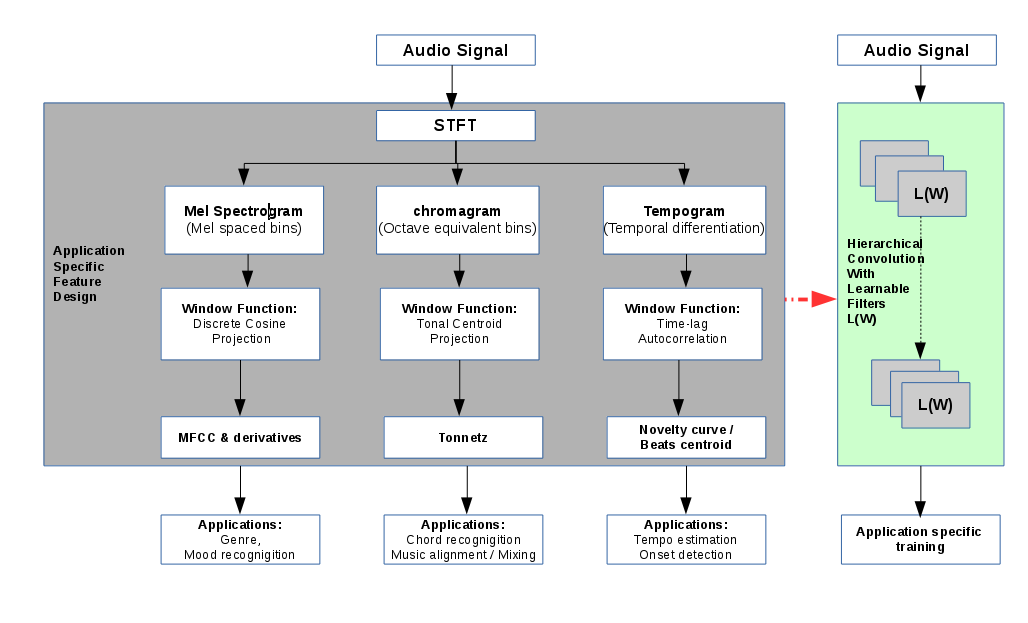
\includegraphics[width=0.95\textwidth]{dnn_motivation}
\caption{Motivation for deep architectures}
 \label{fig:deep learning}
 \end{figure}
\FloatBarrier
\bigskip

\section{Temporal pooling}
\label{temporal}
\subsection{Clustering}
\label{clustering}
\subsection{Recurrent Neural Networks}
\label{rnn}

\section{Training}
\label{training}
}
